%%%%%%%%%%%%%%%%%%%%%%%%%%%%%%%%%%%%%%%%%
% Wenneker Assignment
% LaTeX Template
% Version 2.0 (12/1/2019)
%
% This template originates from:
% http://www.LaTeXTemplates.com
%
% Authors:
% Vel (vel@LaTeXTemplates.com)
% Frits Wenneker
%
% License:
% CC BY-NC-SA 3.0 (http://creativecommons.org/licenses/by-nc-sa/3.0/)
% 
%%%%%%%%%%%%%%%%%%%%%%%%%%%%%%%%%%%%%%%%%

%----------------------------------------------------------------------------------------
%	PACKAGES AND OTHER DOCUMENT CONFIGURATIONS
%----------------------------------------------------------------------------------------

\documentclass[11pt, parskip=half]{scrartcl} % Font size

%%%%%%%%%%%%%%%%%%%%%%%%%%%%%%%%%%%%%%%%%
% Wenneker Assignment
% Structure Specification File
% Version 2.0 (12/1/2019)
%
% This template originates from:
% http://www.LaTeXTemplates.com
%
% Authors:
% Vel (vel@LaTeXTemplates.com)
% Frits Wenneker
%
% License:
% CC BY-NC-SA 3.0 (http://creativecommons.org/licenses/by-nc-sa/3.0/)
% 
%%%%%%%%%%%%%%%%%%%%%%%%%%%%%%%%%%%%%%%%%

%----------------------------------------------------------------------------------------
%	PACKAGES AND OTHER DOCUMENT CONFIGURATIONS
%----------------------------------------------------------------------------------------

\usepackage{amsmath, amsfonts, amsthm} % Math packages

\usepackage{geometry}

\usepackage{listings} % Code listings, with syntax highlighting

\usepackage[french]{babel} % English language hyphenation

\usepackage{graphicx} % Required for inserting images
\graphicspath{{Figures/}{./}} % Specifies where to look for included images (trailing slash required)

\usepackage{booktabs} % Required for better horizontal rules in tables

\usepackage{subcaption} % Required for creating figures with multiple parts (subfigures)

\usepackage{todonotes} % Required for inserting todo notes

\usepackage{array} % Required for customising tables

\usepackage{hyperref} % Required for adding links	and customising them

\numberwithin{equation}{section} % Number equations within sections (i.e. 1.1, 1.2, 2.1, 2.2 instead of 1, 2, 3, 4)
\numberwithin{figure}{section} % Number figures within sections (i.e. 1.1, 1.2, 2.1, 2.2 instead of 1, 2, 3, 4)
\numberwithin{table}{section} % Number tables within sections (i.e. 1.1, 1.2, 2.1, 2.2 instead of 1, 2, 3, 4)

\setlength\parindent{0pt} % Removes all indentation from paragraphs

\usepackage{enumitem} % Required for list customisation
\setlist{noitemsep} % No spacing between list items

%----------------------------------------------------------------------------------------
%	DOCUMENT MARGINS
%----------------------------------------------------------------------------------------

\usepackage{geometry} % Required for adjusting page dimensions and margins

\geometry{
	paper=a4paper, % Paper size, change to letterpaper for US letter size
	top=2.5cm, % Top margin
	bottom=3cm, % Bottom margin
	left=3cm, % Left margin
	right=3cm, % Right margin
	headheight=0.75cm, % Header height
	footskip=1.5cm, % Space from the bottom margin to the baseline of the footer
	headsep=0.75cm, % Space from the top margin to the baseline of the header
	%showframe, % Uncomment to show how the type block is set on the page
}

%----------------------------------------------------------------------------------------
%	FONTS
%----------------------------------------------------------------------------------------

\usepackage[utf8]{inputenc} % Required for inputting international characters
\usepackage[T1]{fontenc} % Use 8-bit encoding

\usepackage{fourier} % Use the Adobe Utopia font for the document

%----------------------------------------------------------------------------------------
%	SECTION TITLES
%----------------------------------------------------------------------------------------

\usepackage{sectsty} % Allows customising section commands

\sectionfont{\vspace{6pt}\centering\normalfont\scshape} % \section{} styling
\subsectionfont{\normalfont\bfseries} % \subsection{} styling
\subsubsectionfont{\normalfont\itshape} % \subsubsection{} styling
\paragraphfont{\normalfont\scshape} % \paragraph{} styling

%----------------------------------------------------------------------------------------
%	HEADERS AND FOOTERS
%----------------------------------------------------------------------------------------

\usepackage{scrlayer-scrpage} % Required for customising headers and footers

\ohead*{} % Right header
\ihead*{} % Left header
\chead*{} % Centre header

\ofoot*{} % Right footer
\ifoot*{} % Left footer
\cfoot*{\pagemark} % Centre footer
 % Include the file specifying the document structure and custom commands
\geometry{a4paper, margin=0.8in}

%----------------------------------------------------------------------------------------
%	TITLE SECTION
%----------------------------------------------------------------------------------------

\title{	
	\normalfont\normalsize
	\large\textsc{Sorbonne Université, UFR de Physique}\\ % Your university, school and/or department name(s)
	\vspace{2pt} % Whitespace
	\normalsize Master 1 : Physique fondamentale et applications\\
	\vspace{25pt} % Whitespace
	\rule{\linewidth}{0.5pt}\\ % Thin top horizontal rule
	\vspace{20pt} % Whitespace
	{\huge Projet IA : Le Modèle d'Ising}\\ % The assignment title
	\vspace{2pt} % Whitespace
	{Intelligence artificielle pour la physique}\\
	\vspace{12pt} % Whitespace
	\rule{\linewidth}{2pt}\\ % Thick bottom horizontal rule
	\vspace{12pt} % Whitespace
}

\author{\LARGE A. Cremel-Schlemer \large (3800159) \\ \LARGE G. Carvalho \large (28709594) \\ \LARGE M. Panet \large (28705836)} % Your name

\date{\normalsize\today} % Today's date (\today) or a custom date

\begin{document}

\maketitle % Print the title
\tableofcontents % Print the contents

\newpage

\addcontentsline{toc}{section}{Introduction}
\section*{Introduction}

Le modèle d'Ising est un modèle de physique statistique introduit par Rudolph Peierls, Wilhelm Lenz et Ernst Ising dans les années 1920. Ce modèle d'une remarquable simplicité lui permet pourtant de mettre en exergue un comportement de transition de phase. \par


Sous sa formulation historique, le modèle d'Ising permet d'étudier la transition de phase paramagnétique/ferromagnétique d'un matériau.
Certains matériaux possèdent une aimantation intrinsèque ; ils sont dits ferromagnétiques. C'est le cas des aimants. Cette propriété provient d'interactions à courte portée entre les spins d'un cristal. Mais, comme l'a découvert en 1895 le physicien Pierre Curie, ces matériaux perdent leur propriété magnétique au-dessus d'une température caractéristique appelée température de Curie $T_C$.
On trouve aussi des matériaux dits paramagnétiques. Ces matériaux ne sont pas magnétiques, mais le deviennent au contact d'un champ magnétique extérieur puissant.
En l'absence de champ magnétique extérieur, les spins de ces matériaux sont désordonnés, de sorte qu'en moyenne, le moment magnétique du matériau est nul : le materiaux n'est pas magnétique. Sous l'action d'un champ magnétique extérieur, ces moments se polarisent, ce qui rend le matériau magnétique.

L'hamiltonien du modèle d'Ising prend donc en compte ces deux propriétés, puisqu'une partie de cet est relative à l'interaction ferromagnétique à courte portée et l'autre partie est relative à l'interaction de chaque spin du cristal avec un champ magnétique extérieur.
Dans la plupart des modèles numériques, on travaille sans champ extérieur.


La relative généralité de ce modèle (interactions locales et interaction individuelle avec une force extérieure) transcende la physique et permet de décrire qualitativement et parfois quantitativement une très grande variété de situations (paramagnétisme, gaz réticulaire, agents économiques, modèles écologiques, utilisation en analyse et traitement de l'image). Il donnera même lieu à un modèle plus général : le modèle de Potts (qui généralise l'aspect binaire du modèle d'Ising lié à la binarité des spins).


À travers notre exposé sur l'intelligence artificielle, nous allons nous intéresser à un jeu de données constitué de $16 000$ images issues d'une simulation numérique du modèle d'Ising 2D. Chaque image est associée à une température caractéristique allant de $0.25$ à $4$ (sans unité) et à un label. Le label renseigne sur la phase dans laquelle l'image se trouve. La \textit{phase ferromagnétique} est une phase où les spins sont globalement tous alignés ou forment des îlots de spins alignés ($|M| > 0$). Le label \textit{phase paramagnétique} rends compte du régime où les spins sont globalement désordonnés ($M = 0$).


Nous allons explorer différentes méthodes pour voir quelles solutions d'intelligence artificielle nous permettent de trancher, à partir d'une image donnée, si l'on est dans la phase paramagnétique ou ferromagnétique. Nous nous intéresserons aussi à la manière dont sont générées les données du modèle d'Ising. Nous chercherons à voir s'il est possible de prédire la température d'une image de manière fiable et même s'il est possible de générer de nouvelles données sans faire appel à une simulation numérique coûteuse.

\section{Génération de données}
Afin de mieux cerner le problème initiale, nous avons recréé la simulation du modèle d'Ising 2D pour des images $40 \times 40$ comme celle présente dans le dataset.
Le modèle d'Ising 2D est une approche numérique du problème posé en introduction où l'on fait l'hypothèse d'un cristal plat et de maille carrée pour lequel chaque atome est associé à un pixel d'une image.


Chaque spin est représenté soit par un 0, soit par un 1. Le 1 pour un spin Up, le 0 pour un spin Down. Pour améliorer la validité du modèle, des conditions aux bords périodiques sont utilisées. Concrètement cela revient à traiter la surface d'un tore qu'on aurait dépliée (cf. Figure \ref{fig:ising2D}).

\begin{figure}[h]
	\begin{subfigure}{0.5\textwidth}
		\centering
		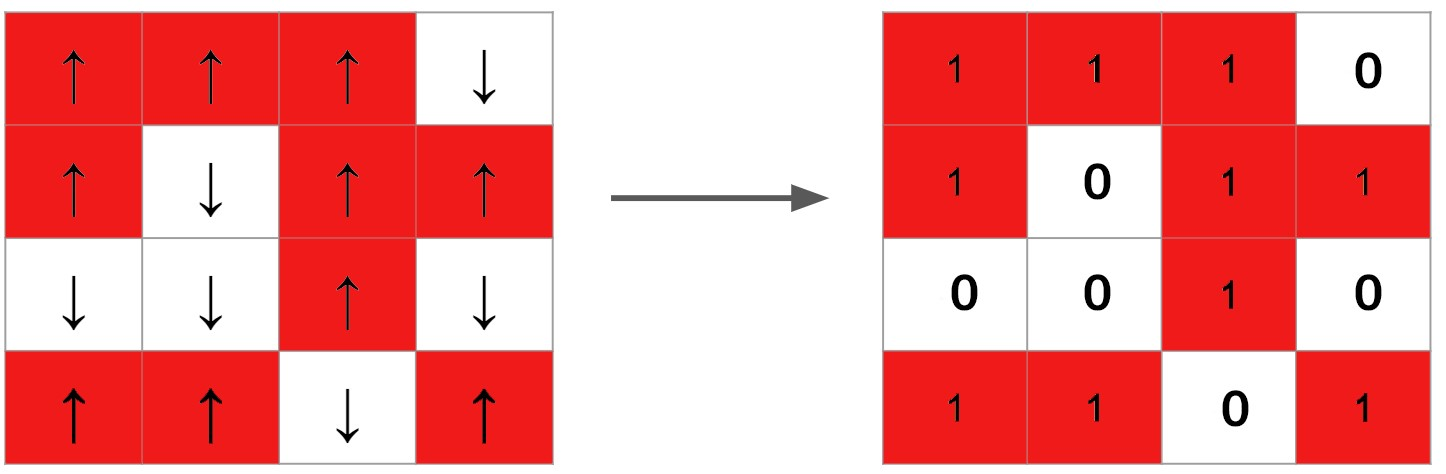
\includegraphics[width=0.95\linewidth]{./figures/torus_left.jpg}
		\caption{Les spins sont soit Up = 1, soit Down = 0}
	\end{subfigure}
	\begin{subfigure}{0.5\textwidth}
		\centering
		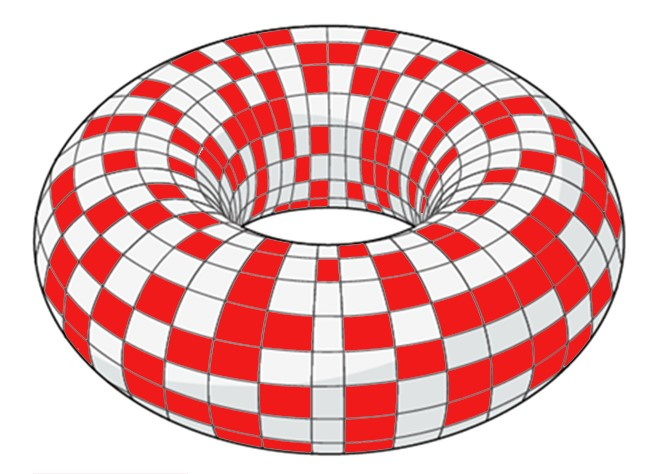
\includegraphics[width=0.5\linewidth]{./figures/torus_right.jpg}
		\caption{Conditions aux bords périodiques}
	\end{subfigure}
	\caption{Représentation du modèle d'Ising 2D}
	\label{fig:ising2D}
\end{figure}


Le Hamiltonien du problème est donnée par l'équation :

\begin{equation*}
	H = -J  \displaystyle \sum_{i,j}\sigma_{i}\sigma_{j} - h\displaystyle \sum_{i} \sigma_{i}
\end{equation*}

où $\sigma_{i} = \pm 1$. Celà dit, comme nous travaillons avec des $0$ et des $1$, il y a quelques manipulations à réaliser sur l'Hamiltonien. On fait de plus abstraction de la deuxième partie de l'hamiltonien qui traite du paramgnétisme.

Il nous reste donc qu'à traiter :
\begin{equation*}
	H = -J  \displaystyle \sum_{i,j}(2\sigma_{i}-1)(2\sigma_{j}-1)
\end{equation*}

Que signifie cet Hamiltonien ? C'est un Hamiltonien de couplage entre spin. À priori, pour respecter la physique du système qu'on cherche à étudier, ce couplage ne se réalise qu'à courte portée, et donc que entre spin "plus proche voisin" puisqu'il s'agit d'une intéraction d'échange à courte portée. Par ailleurs, on choisie de travailler avec des constantes dimentionnées de sorte que: $\frac{J}{K_B}=1$

On va maintenant se rapprocher d'un des spins de notre modèle. Situé au centre, ses plus proches voisins forment une croix suisse autour de lui. On calcule son Hamiltonien local :

\begin{equation*}
	H_{local} = E_{ij} =  (2\sigma_{i}-1) \displaystyle \sum_{j}(2\sigma_{j}-1) = (2\sigma_{i}-1) \times \bigg[ 2\times( R + L + U + D ) -4 \bigg]
\end{equation*}
avec :

\begin{figure}[h]
	\centering
	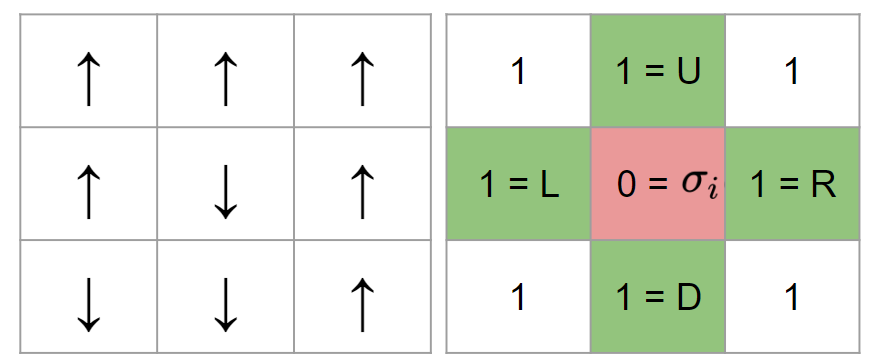
\includegraphics[width=0.5\linewidth]{H.png}
	\caption{Hamiltonien local}
	\label{fig:H}
\end{figure}

Partons d'un système idéal où tous les spins sont alignées. En raison de l'agitation thermique un spin aléatoire du cristal inverse son sens. La variation d'énergie associé à ce changement est donnée par :
\begin{equation*}
	\Delta E = E_f - E_i
\end{equation*}
Et la probabilité qu'un tel changement s'opère est proportionelle au poids de Boltzmann :

\begin{equation*}
	P(\Delta E) \propto e^{-\beta \Delta E} = e^{-\beta \Delta E}
\end{equation*}

L'idée est la suivante :  l'ordinateur va piocher une case au hasard calculer le $\Delta E$ associé. Ce $\Delta E$ ne peux prendre que 5 valeurs possibles :
\begin{center}
	\begin{tabular}{|l|m{4cm}|}
		\hline
		n voisin de sens opposé & $\Delta E $ \\
		\hline
		0                       & 8           \\
		1                       & 4           \\
		2                       & 0           \\
		3                       & -4          \\
		4                       & -8          \\\hline
	\end{tabular}
\end{center}

\vspace{4mm}

Dans le cas ou $\Delta E \in \{0,-4,-8\}$ l'energie est minimisée donc le changement s'opère naturellement, l'ordinateur change le pixel d'état.
Dans le cas inverse, c'est à dire  $\Delta E \in \{4,8\}$ un nombre aléatoire $x$ tiré selon une distribution uniforme entre 0 et 1 et est comparer à $e^{-\beta \Delta E}$.
Si $x < e^{-\beta \Delta E}$ alors l'ordinateur change le pixel d'état. Sinon il ne le fait pas.

On remarque que plus T est important plus la probabilité de transition est importante.

\begin{figure}[h]
	\centering
	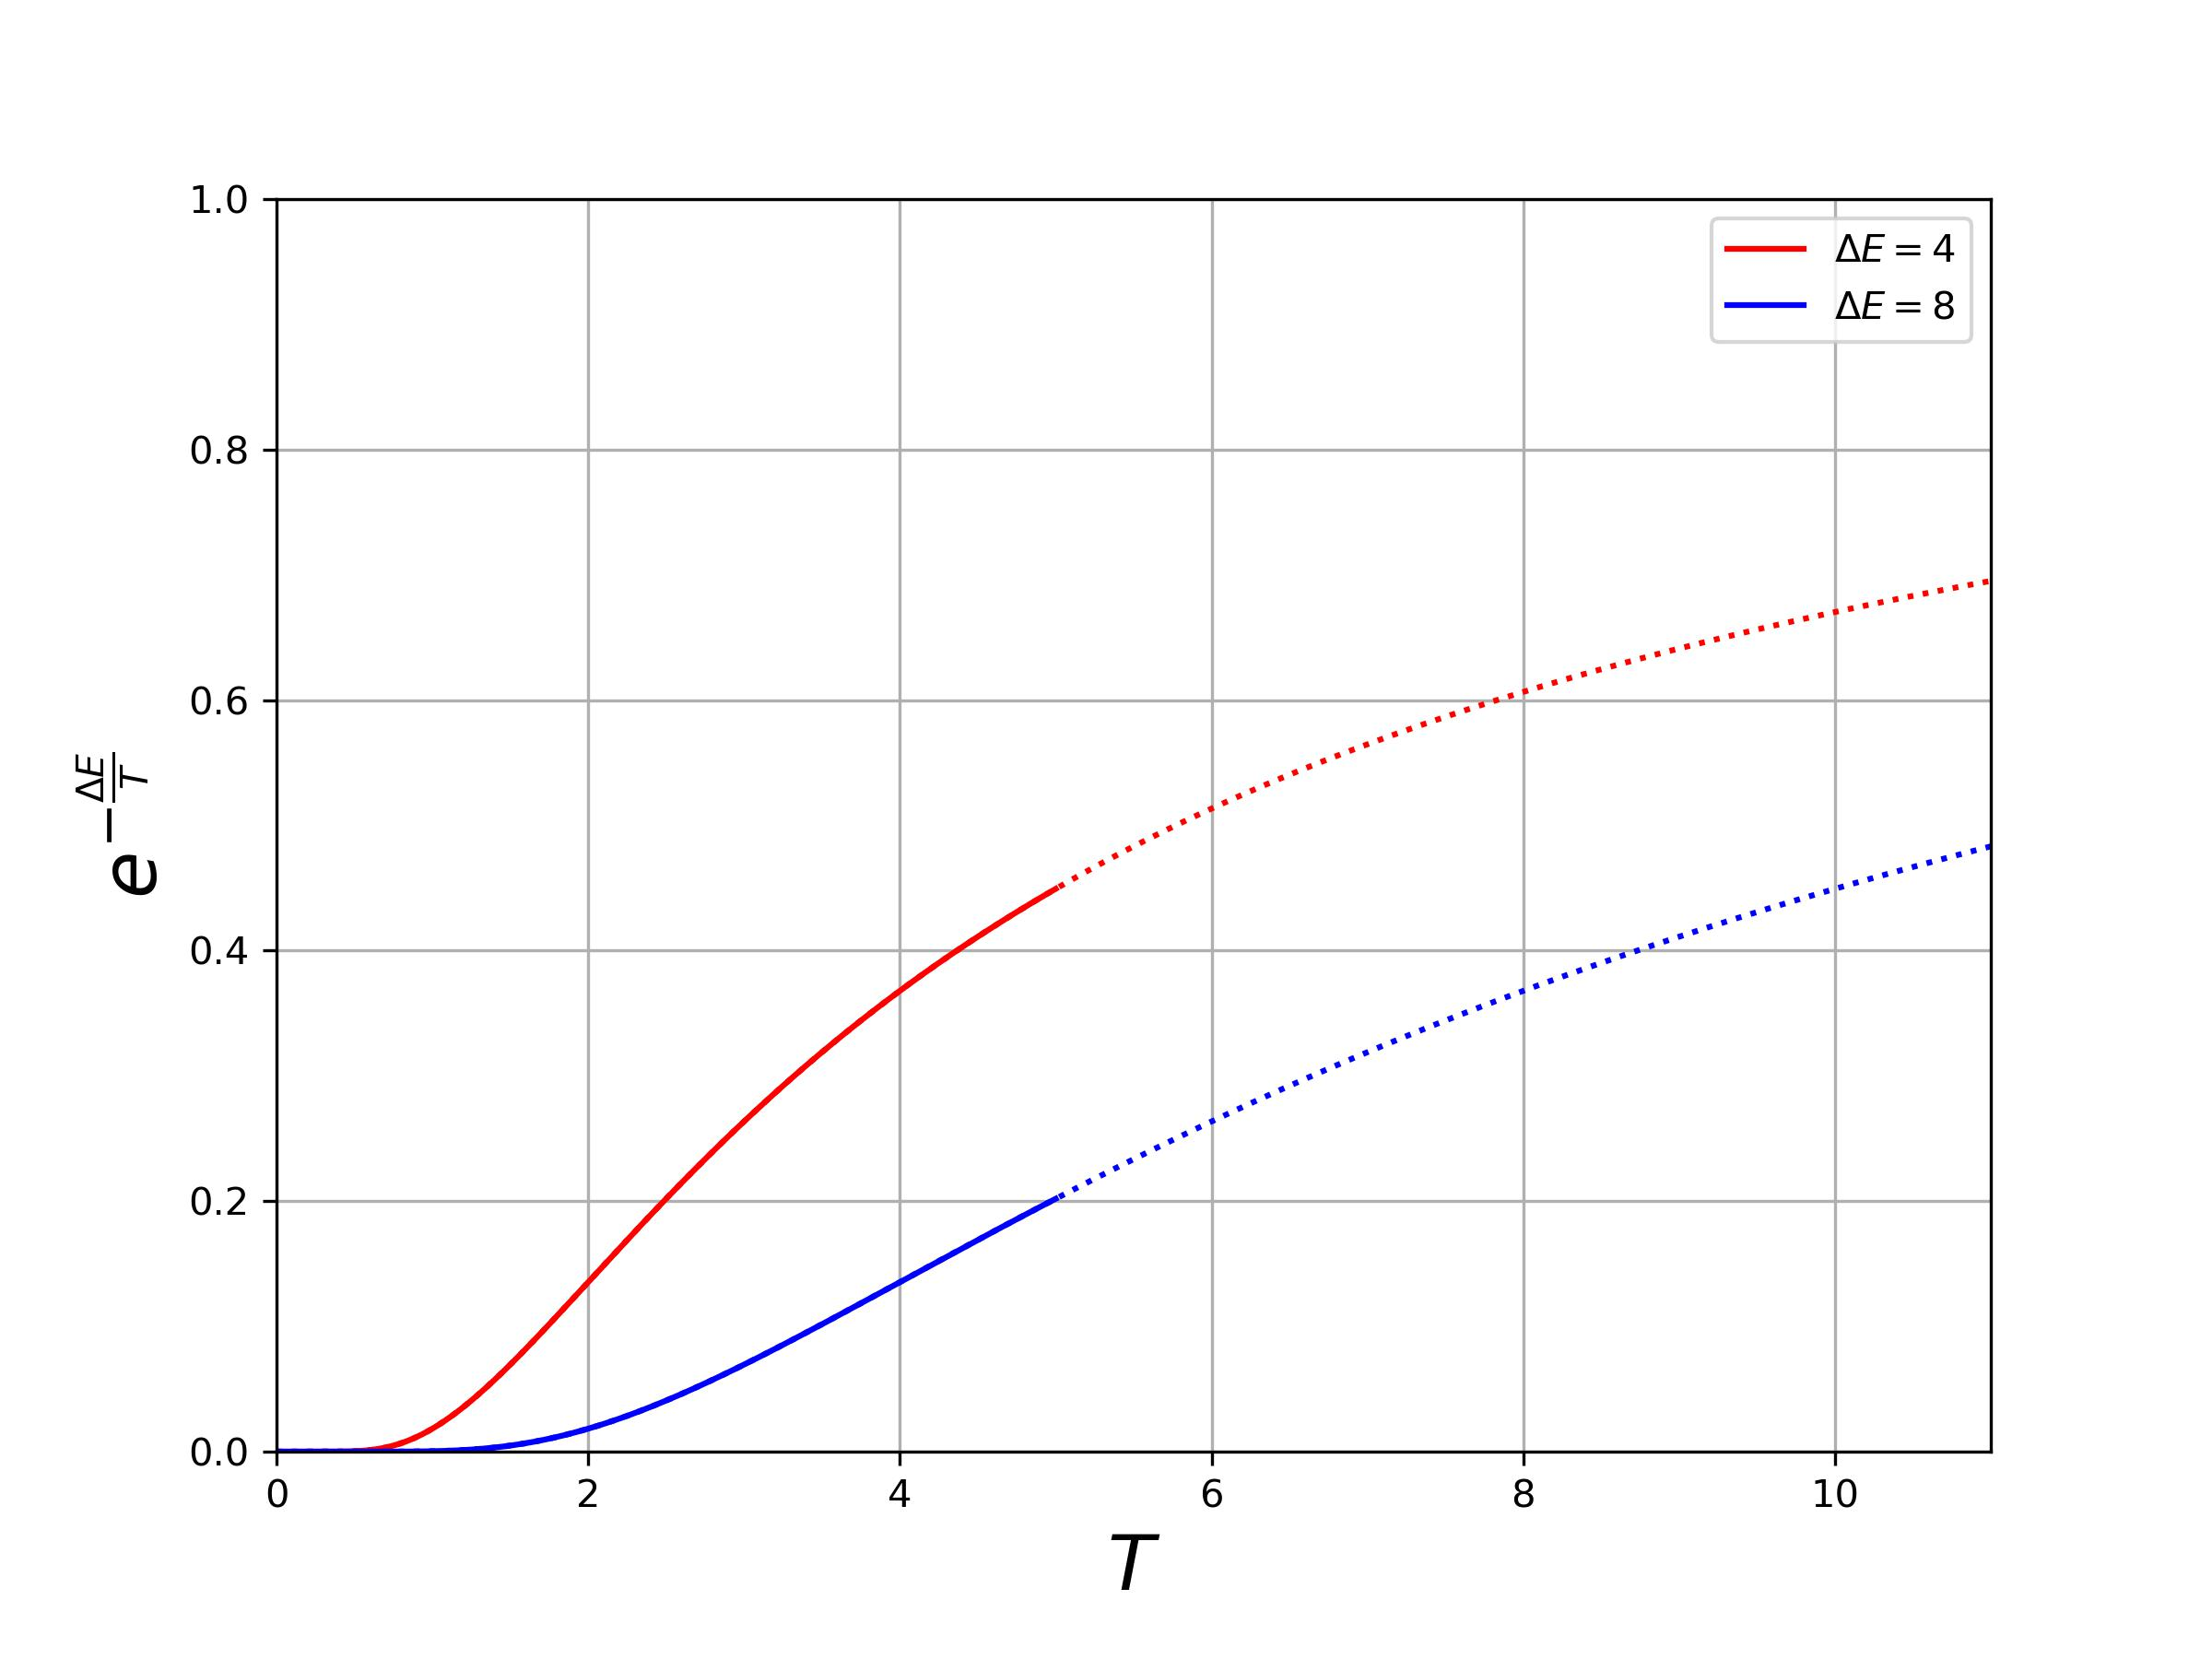
\includegraphics[width=0.5\linewidth]{proba.jpg}
	\caption{probabilité de transition en fonction de la température}
	\label{fig:H}
\end{figure}

On peut donc alors lancer la simulation, pour une température fixé on réalise un certains nombre de tentative de changement de spin. Le système va alors se relaxer jusqu'à un équilibre où la moyenne des spins qui composent l'image est stable tentative successive de changement de l'état d'un spin de l'image.

\begin{figure}[h]
	\centering
	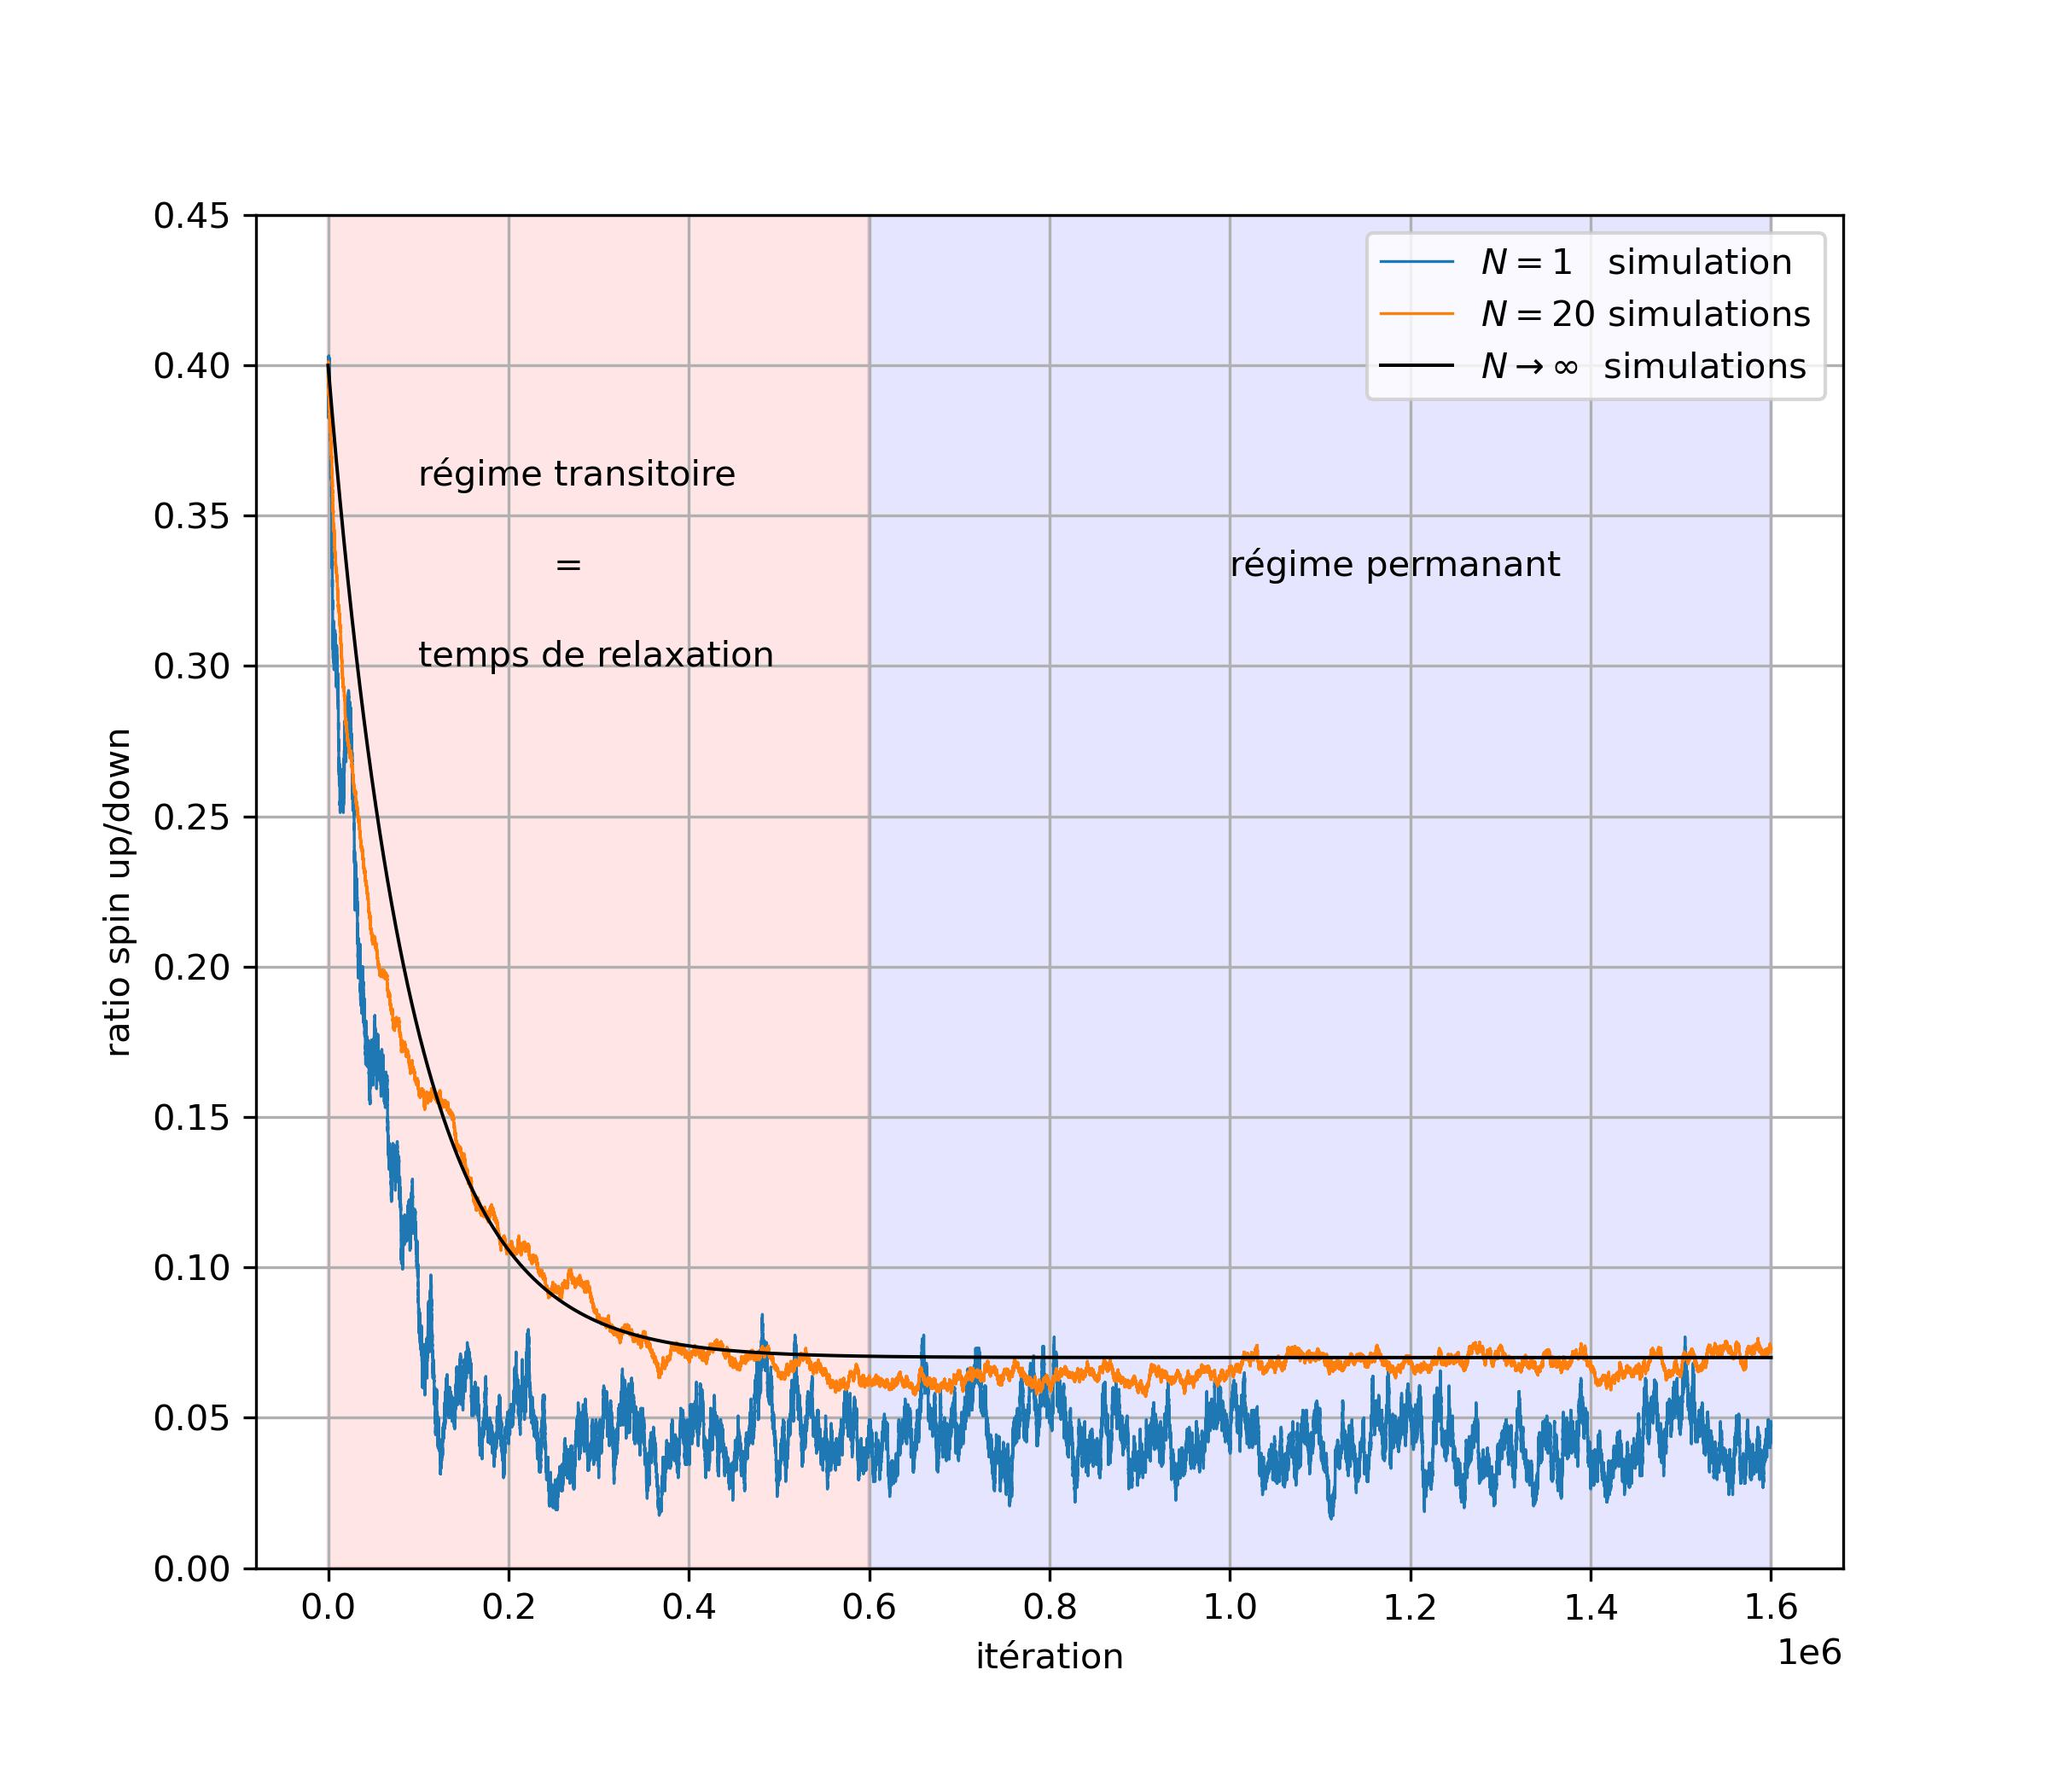
\includegraphics[width=0.5\linewidth]{simulation_ising.jpg}
	\caption{Évolution du ratio spin up spin down pour $T=2$ et $1,6$ million itération }
	\label{fig:H}
\end{figure}


\section{Pré-traitement des données}
Maintenant que nous avons généré nos données, nous devons nous faire une idée de la forme de nos données afin de pouvoir les traiter de la meilleure façon possible.
Les données fournies au départ sont des vecteurs de taille $1600$ contenant des $1$ et des $0$. Ces vecterus représentent des configurations de spins se trouvant sur une grille 2D de taille $40 \times 40$. Le dataset original est composé de $10000$ configurations de spins pour $16$ températures différentes comprises entre $0.25$ et $4.00$ avec un pas de $0.25$.
Avec ces configurations, un label est associé à chaque configuration. Ce label est une valeur binaire qui nous indique la phase dans laquelle se trouve le système.
De plus, nous avons généré un second jeu de données avec \todo{change number}$X$ configurations de spins pour \todo{change number}$Y$ températures comprises entre $0.25$ et $4.00$. Ce second jeu de données nous permettra de tester nos modèles sur des données avec des températures différentes de celles du jeu de données original. On pourra ainsi voir si nos modèles sont capables de se séparer des températures discrètes du jeu de données original.
Comme on peut le voir sur la figure \ref{fig:rawdata}, nos données forment un ensemble bruité mais il apparaît une symétrie par rapport à l'axe horizontal. En effet, à basse température, les spins sont majoritairement alignés de la même façon mais de manière aléatoire en $+$ ou $-$.
Cette symétrie de nos données peut poser un problème à nos modèles qui auront dû apprendre à faire la différence entre deux configurations opposées mais équivalentes. Pour éviter ce problème, nous allons symétriser nos données en inversant les spins de toutes les configurations qui ont une moyenne de spin négative.
Ainsi, on se retrouve avec des données symétriques par rapport à l'axe horizontal comme on peut le voir sur la figure \ref{fig:symdata}.

\begin{figure}[h]
	\begin{subfigure}{0.5\textwidth}
		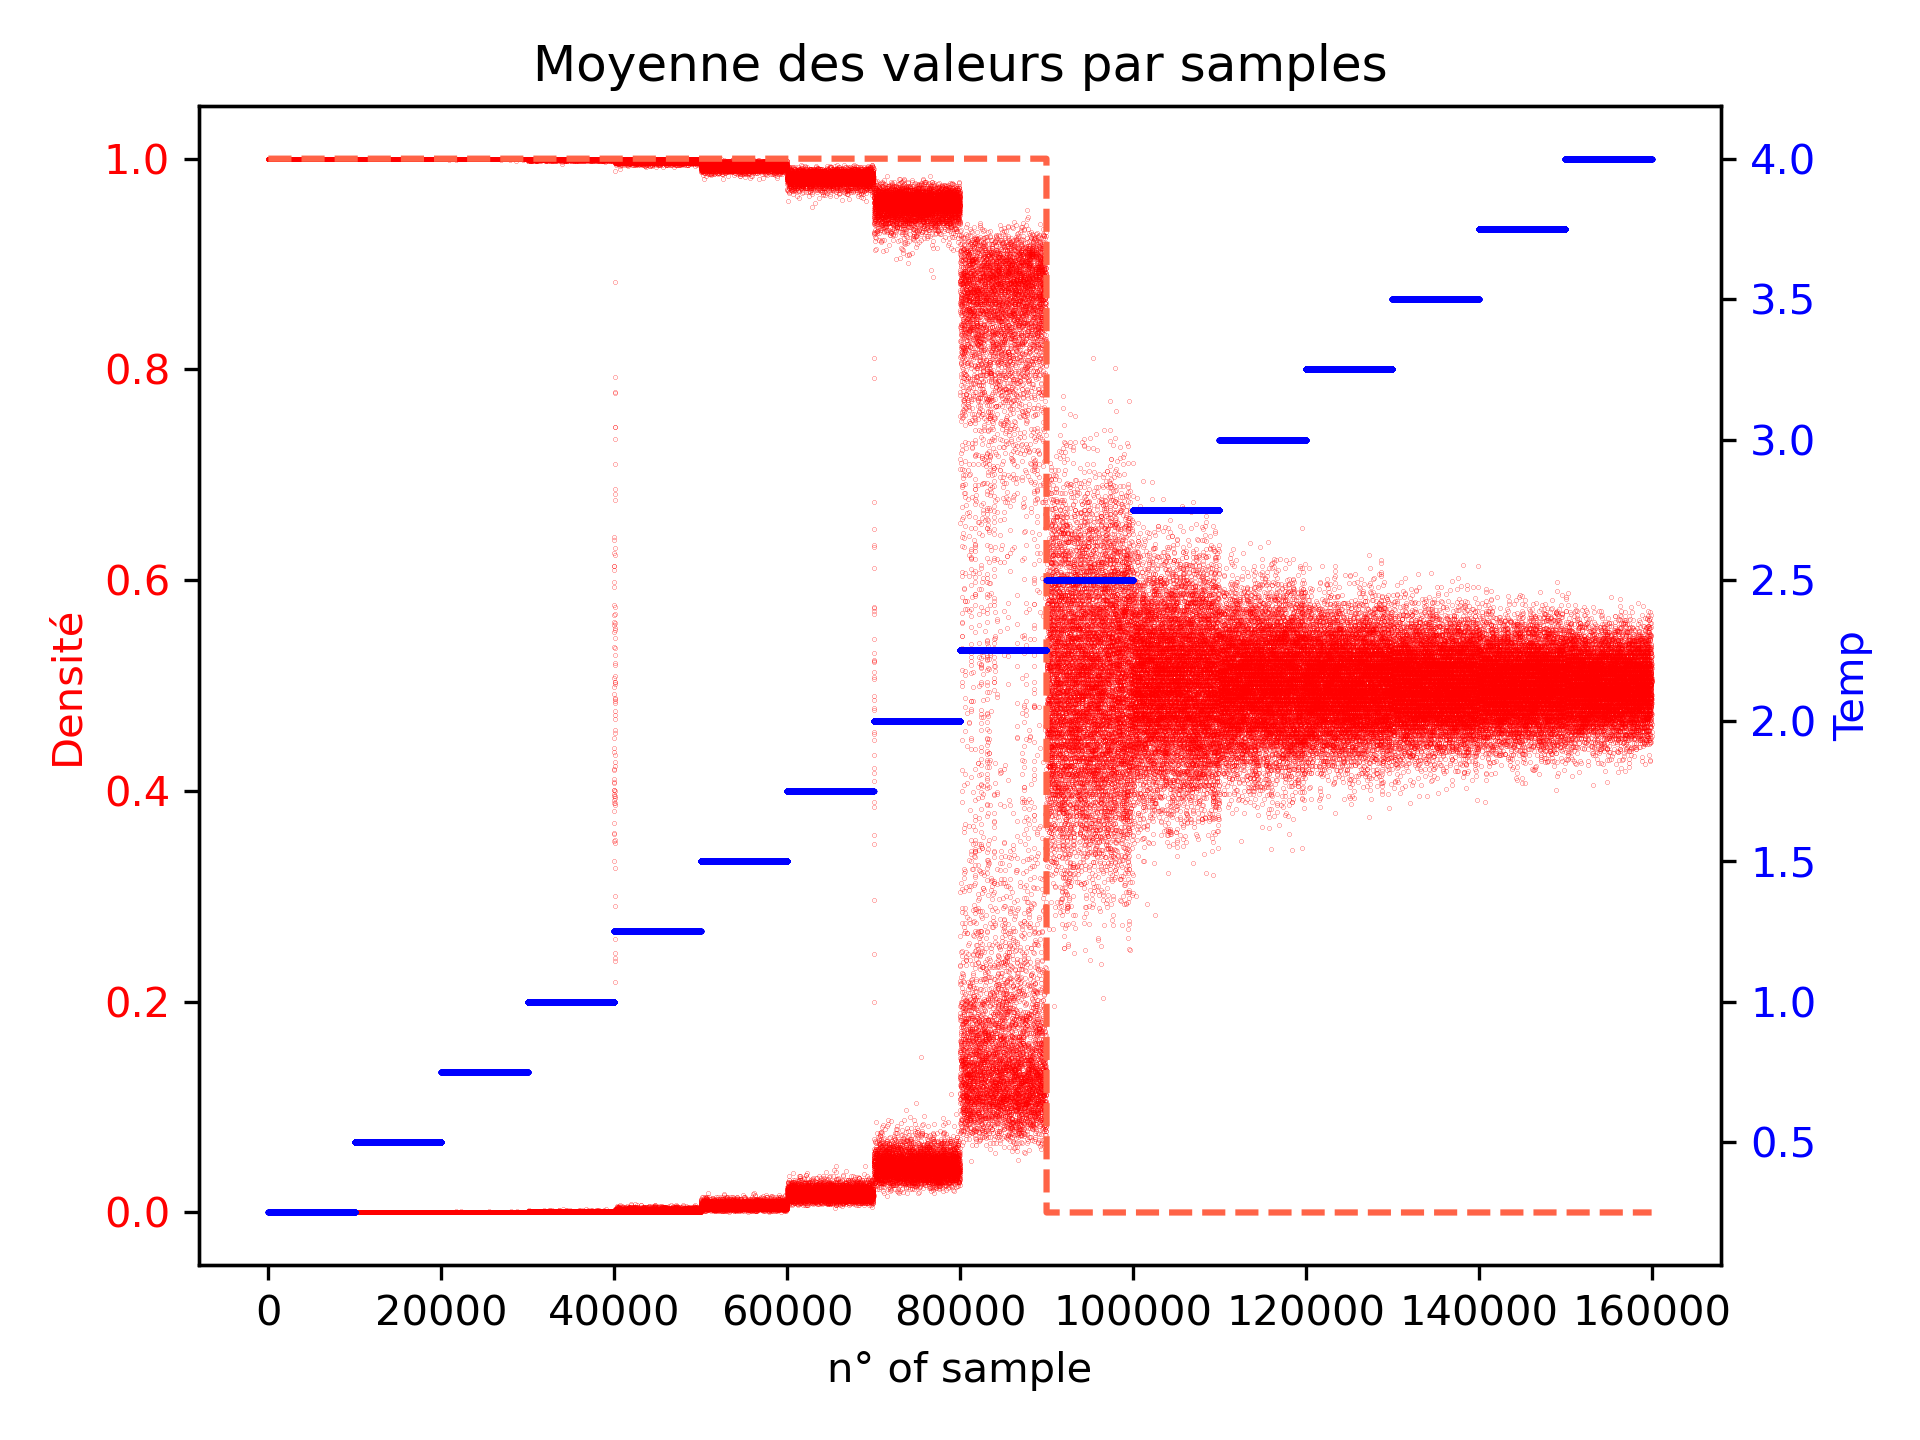
\includegraphics[width=0.95\linewidth]{./figures/raw_data.png}
		\caption{Données brutes}
		\label{fig:rawdata}
	\end{subfigure}
	\begin{subfigure}{0.5\textwidth}
		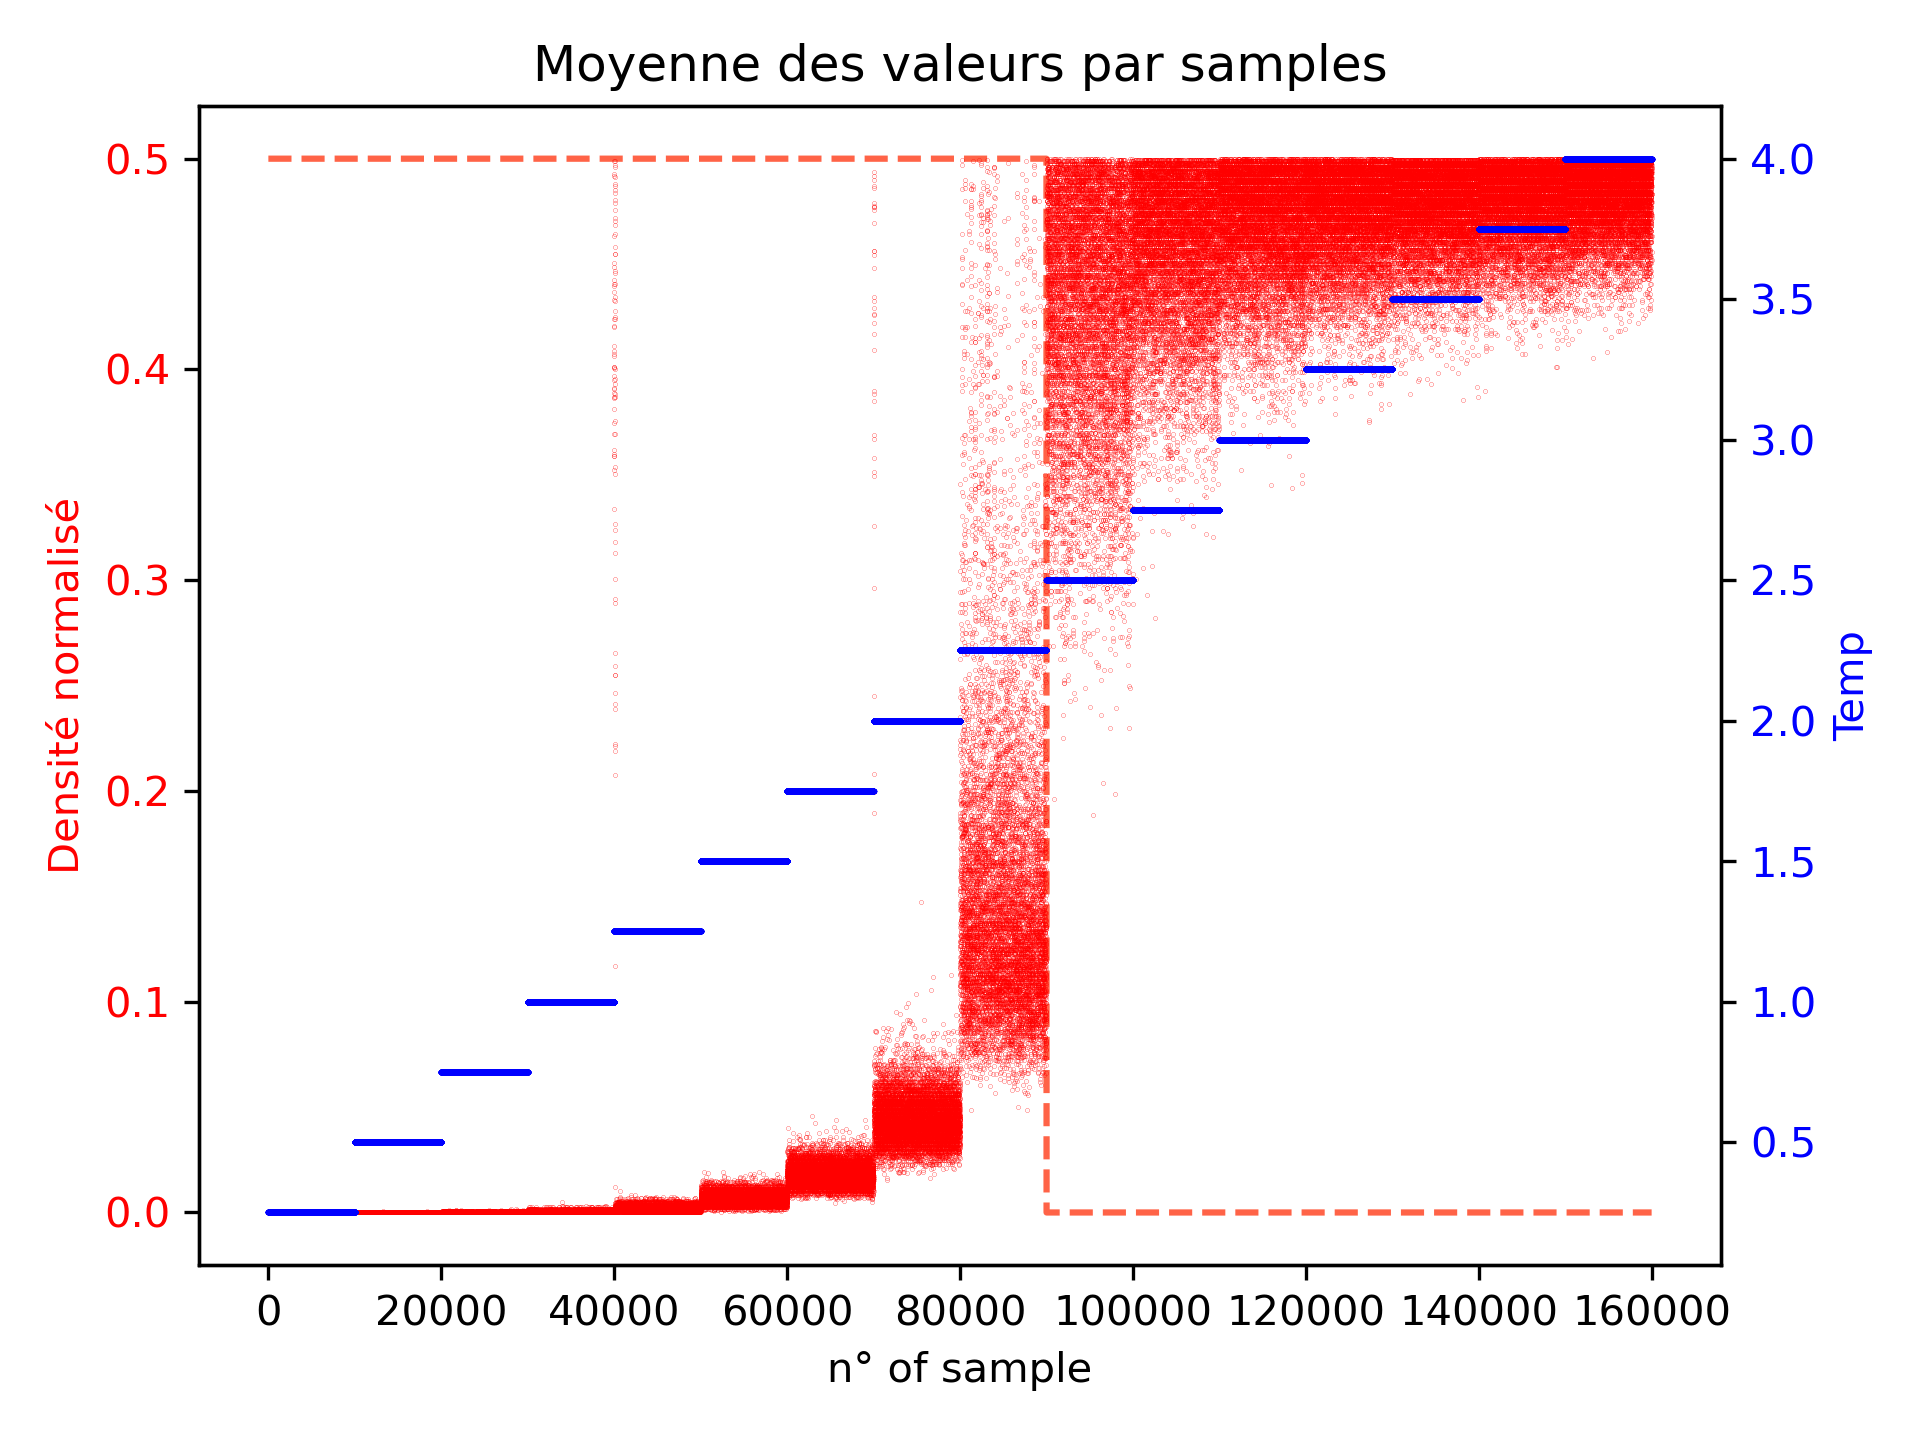
\includegraphics[width=0.95\linewidth]{./figures/sym_data.png}
		\caption{Données symétrisées}
		\label{fig:symdata}
	\end{subfigure}
	\caption{}
\end{figure}

Dans la partie suivante, nous allons entraîner certains modèles spécifiques sur la densité de spin symétrisée. Dans ce cas, nous allons aussi normaliser afin de rendre les modèles plus performants.
Pour cela, nous allons utiliser la méthode \textit{StandardScaler} de la librairie \textit{sklearn} qui permet de centrer et réduire les données. Cette méthode soustrait la moyenne et divise par l'écart-type. Ainsi, on se retrouve avec des données centrées en $0$ et de variance $1$.

Afin d'appliquer exactement la même transformation sur les données de test, nous allons créer un pipeline qui va appliquer la méthode de symétrisation puis la méthode de normalisation. Ainsi, on pourra appliquer le pipeline sur les données de test sans avoir à les modifier.
Finalement, certains modèles seront plus réceptifs à des données présentées sous forme de vecteur de taille $1600$, d'autre sous forme de matrice de taille $40 \times 40$. Pour éviter de devoir modifier les données à chaque fois, nous allons créer un pipeline qui va transformer les données en matrice si nécessaire et appliquer les autres méthodes de pré-traitement expliquées ci-dessus.

\section{Modèles classiques}

\subsection{Analyse par la magnétisation}
Notre première approche de ce problème est de considérer la magnétisation comme une fonction de la température. Cette approche nous permet de réduire grandement la complexité du problème. En effet, nous n'avons plus qu'une seule variable à considérer : l'état moyen des spins. Dans cette partie, nous allons donc essayer de prédire la température à partir de la magnétisation. Il suffit ensuite de comparer la valeur prédite à la valeur de la température critique pour déterminer la phase du système.

Avant tous, nous allons établir un modèle naif qui va nous servir de référence. Ce modèle va simplement renvoyer la valeur moyenne de la température du jeu de données. Ainsi, on pourra comparer les performances de nos modèles avec ce modèle naif. On obtient une erreur quadratique moyenne de $1.32$.

Du fait du bruit de nos données et du faible nombre de températures distinctes, nous devons porter une attention particulière au sur-apprentissage de nos modèles.
Prenant en compte le grand nombre de données, nous sommes partis sur un modèle de foret aléatoire. Ce modèle est très robuste et permet de limiter le sur-apprentissage. De plus, il est très rapide à entraîner et à tester.
Au niveau des hyperparamètres, nous avons limité la profondeur des arbres à 5 et nous avons aussi composé la foret de $100$ arbres. De plus, la méthode de \textit{Bootsrap} est activée. Cette méthode permet de créer des sous-ensembles de données de la taille de l'ensemble de données originale. Ainsi, on peut entraîner plusieurs arbres sur des données différentes et les combiner pour obtenir un modèle plus robuste.
On peut donc limiter le sur-apprentissage tout en gardant un modèle performant. Les résultats obtenus sont présentés sur la figure \ref{fig:forest}.
La figure \ref{fig:forest} possède deux objets : La densité de points de la moyenne des spins symétrisée par température calculé en utilisant la méthode de \textit{kde} et la prédiction du modèle de foret aléatoire.

Avec une MSE de $0.108$, on obtient un modèle qui est $12$ fois plus performant que le modèle naif. Cependant, on peut voir que le modèle a du mal à distinquer les hautes températures. En effet, les valeurs prédites par ce modèle sont toujours inférieures à $3.5$.
Cela peut s'expliquer par le fait que, à haute température, la densité est quasiment nulle. Ainsi, lorsque le modèle va essayer de prédire une configuration de spin à haute température, il va prédire la température correspondant plus ou moins à la moyenne des températures capable de produire une configuration de spin similaire. Cela apparaît clairement sur la figure \ref{fig:forest}.

\begin{figure}[h]
	\centering
	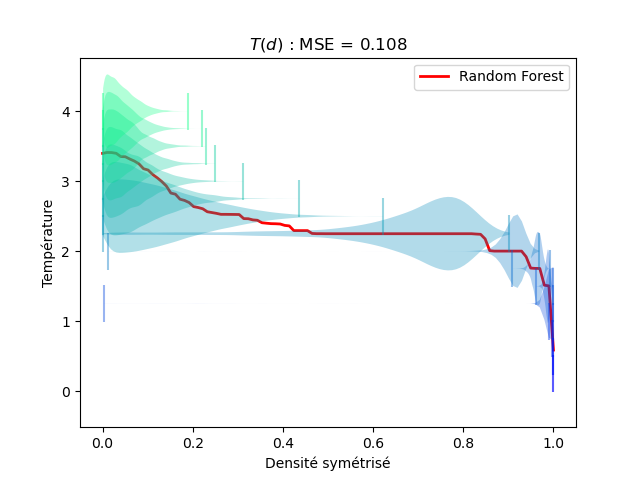
\includegraphics[width=0.75\linewidth]{./figures/forest.png}
	\caption{Résultats du modèle de foret aléatoire}
	\label{fig:forest}
\end{figure}

\subsection{Analyse par l'état individuel des spins}

\section{Réseaux de neurones}
\subsection{Objectif}
Dans le cadre de ce projet, notre objectif final était de développer un modèle performant capable de classer des matrices de taille 40x40 en deux catégories distinctes. Comme dans le modèle d’Ising l’état d’un spin est dépendant de ces plus proches voisins, le plus naturel était de créer un réseau neuronal convolutif car il prend en compte les corrélations locales entre pixels voisins. La performance de notre classification est alors dépendante de l’architecture de notre modèle, de la manière dont il extrait et apprend les caractéristiques pertinentes des matrices en entrée.

Dans cette partie, nous allons analyser l’architecture du modèle qu’on a créé. On va discuter pourquoi on a choisi chaque couche et quel rôle elles jouent dans notre modèle. On analysera ensuite nos étapes d’entraînement puis on discutera les méthodes que nous avons utilisé pour évaluer nos performances.

\subsection{Préparation des données}
\todo{section à compléter}

\subsection{Architecture du modèle}
L’ensemble de l’architecture repose sur des principes de convolution, pooling et de couches entièrement connectées. La combinaison de ces différentes couches crée une architecture cohérente et un modèle performant.

Notre modèle commence par une première couche de convolution 2D, qui utilise 16 filtres de taille 5x5. Cette couche veut extraire des caractéristiques de bas-niveau, soit des bords ou des formes simples présentes dans les données. Cette première couche de convolution est suivie d’une couche de max pooling qui permet, en faisant un sous-échantillonnage, de compresser l’information que l’on veut faire passer à la couche suivante.

On applique ensuite à nouveau ce processus : on a une deuxième couche de convolution 2D a 32 filtres de taille 3x3 et une nouvelle couche de max pooling. Avec cette deuxième couche de convolution, on souhaite capturer des motifs plus complexes et abstraits. On a augmenté le nombre de filtres de la première couche de convolution car on veut augmenter la capacité du modèle : chaque filtre pourra se spécialiser dans la détection de certaines caractéristiques et donc le modèle apprendra plus de relations complexes. Avec la couche de max pooling, on souhaite réduire davantage la dimension spatiale. Finalement, on utilise une dernière couche de convolution 2D avec 64 filtres de taille 3x3, suivie encore d’une autre opération de max pooling.

Ensuite, on utilise une couche Flatten pour aplatir les caractéristiques et motifs extraits de nos couches de convolution pour réduire la dimension de notre matrice. Il s’agit d’une opération assez simple avant d’introduire des couches entièrement connectées Dense. On a utilisé trois couches consécutives : la première avec 128 neurones, la deuxième avec 64 neurones puis la troisième avec 128 neurones. Ces trois couches ont comme objectif d’apprendre les complexités des caractéristiques extraites, afin de réaliser l’objectif de notre modèle. Notre deuxième couche Dense a moins de neurones pour réduire les dimensions et additionner encore un peu de complexité à notre modèle, afin de tout bien représenter. Cette architecture que nous avons utilisée permet une certaine flexibilité au modèle et de s’adapter à la tâche de la classification binaire.

Finalement, l’architecture de notre modèle se termine par une couche de sortie avec une seule cellule, activée à la fonction d’activation sigmoïde. Cela nous permet d’obtenir à la sortie de notre modèle une probabilité que notre sortie appartienne à la classe positive, ce qui correspond bien à ce qui est attendu lors d’une classification binaire.

L’architecture de notre modèle est présentée sous forme d’image dans la figure \ref{fig:model}

\begin{figure}
	\centering
	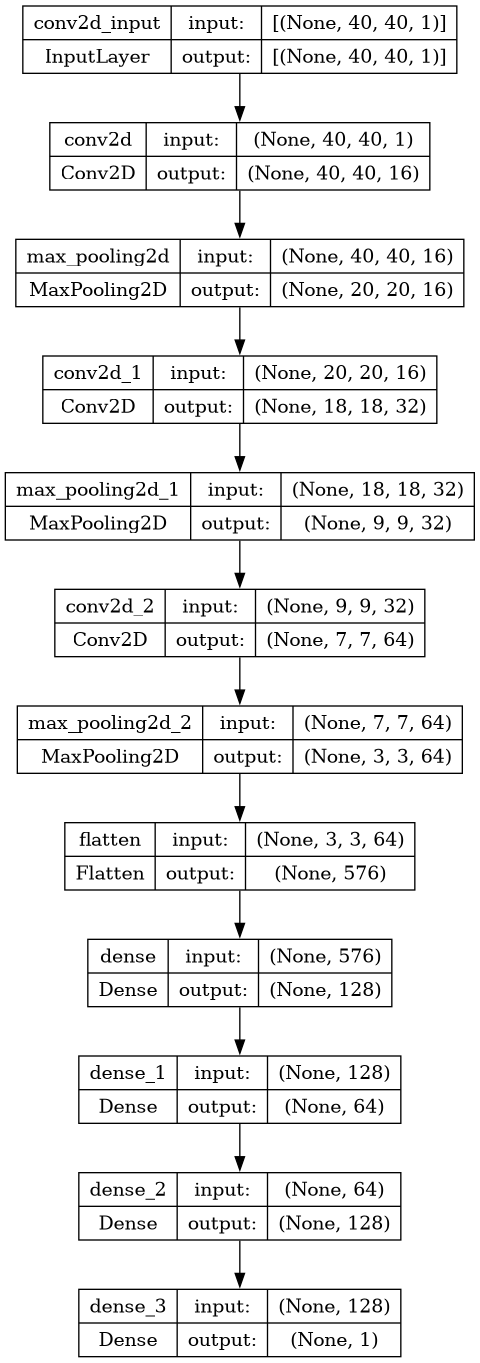
\includegraphics[width=0.4\linewidth]{./figures/model.png}
	\caption{Architecture du modèle}
	\label{fig:model}
\end{figure}

\subsection{Entraînement du modèle}
La procédure d’entraînement consiste à entraîner le modèle à réaliser une classification binaire : identifier s’il y a eu une transition de phase par rapport aux matrices qui décrivent notre système. Avant l’entraînement, nous avons compilé notre modèle avec l’algorithme optimiseur Adam et on a utilisé binary crossentropy comme fonction de coût, une fonction de coût très efficace pour les tâches de classification binaire qui mesure la différence entre les prédictions binaires et les vrais résultats. Finalement, l’entraînement de notre modèle a duré que 11 epochs, avec un batch size de 128. Notre entraînement a duré que 11 epochs pour éviter le sur-apprentissage, puisque nous avons utilisé la méthode de l’arrêt anticipé (early stopping), avec une patience de 5. L’entraînement du modèle a été fait avec les $160 \ 000$ matrices que l'on nous as fournies et a pris que 40 secondes.

Pendant l’entraînement, l’erreur d’entraînement et l’erreur de validation sont enregistrés pour chaque epoch. Cela nous permet de suivre l’entraînement de notre modèle et de détecter des signes de sur-apprentissage ou sous-apprentissage. En suivant cette approche et cette architecture, nous sommes parvenus à un modèle très efficace, dont nous allons étudier les performances maintenant.

\subsection{Evaluation des performances du modèle}
L’objectif principal du modèle est de capturer des motifs complexes qui permettront au modèle d’apprendre les complexités de nos matrices données en entrée et puis faire des prédictions sur à quelle classe appartient chaque matrice. Avec l’enregistrement de l’entraînement et la possibilité de faire des essais avec notre jeu de test, on peut évaluer notre modèle.

Tout d’abord, on peut analyser la performance de notre modèle en prenant en compte l’erreur de la fonction coût sur l’ensemble de données de validation, qui est de seulement \todo{comparer aux autres modèles} 0.0084. Cela indique que le modèle est très performant : il a atteint un niveau très bas de perte sur les données de validation et a une très bonne capacité de se généraliser à de nouvelles données. On peut aussi vérifier la précision (accuracy) de notre modèle sur les données de test : 0.99. Notre modèle est capable de classer correctement 99\% des échantillons dans l’ensemble de test. Cela renforce à nouveau l’idée que notre modèle a une très bonne capacité à généraliser et qu’il est très adéquat à la classification binaire. Nous avons aussi calculé une autre métrique intéressante : la sensibilité, mesurant la capacité du modèle à identifier tous les exemples positifs réels dans l'ensemble de données et nous trouvons une valeur de 0.99, indiquant une excellente capacité à mesurer des vrais positifs.

Ensuite, nous pouvons étudier l’entraînement de notre modèle. Dans la figure \ref{fig:train}, nous observons l’évolution de l’erreur de la fonction de coût des données d’entraînement et de validation au cours de l’entraînement (graphe en haut). On remarque que les courbes représentant ces données sont très proches dès la première epoch jusqu’à l’epoch 6 et puis commencent à diverger ce qui peut être un signe de sur-apprentissage. Cependant, cela peut être négligeable dû à la simple différence de 0.005 entre les deux courbes. On souligne encore que l’évolution de l’entraînement est très légère, sans grande amélioration de l’erreur sur la fonction de coût. Encore dans la figure \ref{fig:train}, on observe l’évolution de la précision au cours de l’entraînement (graphe en bas). On remarque que dès la première epoch jusqu’à la fin de l’entraînement, ces deux courbes sont toujours très proches autour de 0.998, ce qui confirme à nouveau excellente précision de notre modèle.

\begin{figure}[h]
	\centering
	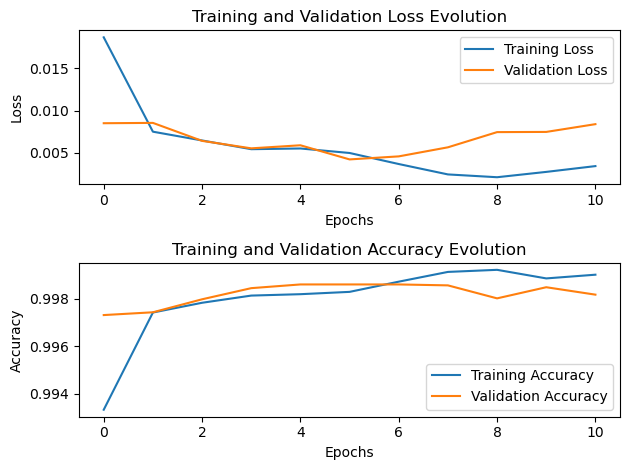
\includegraphics[width=0.66\linewidth]{./figures/train.png}
	\caption{Évolution de l'entraînement}
	\label{fig:train}
\end{figure}

De plus, nous pouvons établir la matrice de confusion de notre modèle, que nous pouvons observer à la figure \ref{fig:matrix}. La matrice de confusion résume le nombre de prédictions correctes et incorrectes faites par le modèle sur l’ensemble des données de test. On observe les vrais négatifs et les vrais positifs, représentés respectivement en haut à gauche et en bas à droite de la matrice de confusion. Ces nombres représentent les prédictions correctes du modèle, où il a réussi à identifier correctement les instances des deux classes,  c’est-à-dire s’il y avait une transition de phase ou pas. Lors des prédictions sur le jeu de test, nous avons 14 158 vrais négatifs (nombre d’échantillons qui étaient réellement dans la classe 0 et correctement identifiés par le modèle) et 17 781 vrais positifs (classe 1 correctement identifiée). De plus, on peut encore observer les faux négatifs et les faux positifs, représentés respectivement en bas à gauche et en haut à droite de la matrice de confusion. Ils représentent les erreurs de classification du modèle. On a 36 faux négatifs et 23 faux positifs, ce qui est négligeable face au nombre de prédictions correctes. Le modèle créé est alors extrêmement efficace à prédire la transition de phase.

\begin{figure}[h]
	\centering
	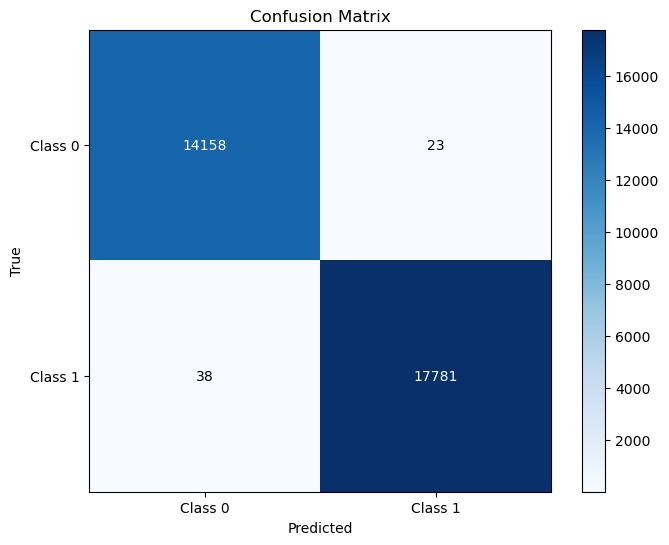
\includegraphics[width=0.5\linewidth]{./figures/matrix.png}
	\caption{Matrice de confusion}
	\label{fig:matrix}
\end{figure}

Finalement, nous pouvons tracer la courbe ROC (Receiver Operating Characteristic), vu dans la figure \ref{fig:ROC}. Il s’agit d’un autre outil d’évaluation de la performance d’un modèle de classification binaire. Elle représente graphiquement la relation entre le taux de vrais positifs, connu aussi comme la sensibilité (ou recall) et le taux de faux positifs lorsqu’on fait varier le seuil de classification. On observe qu’on obtient un AUC (Area Under Curve) de 1.00, ce qui nous indique une performance exceptionnelle de notre modèle. Une valeur de 1.00 signifie une séparation parfaite des classes. Le modèle est très précis dans sa capacité à distinguer les exemples positifs des négatifs.

\begin{figure}[h]
	\centering
	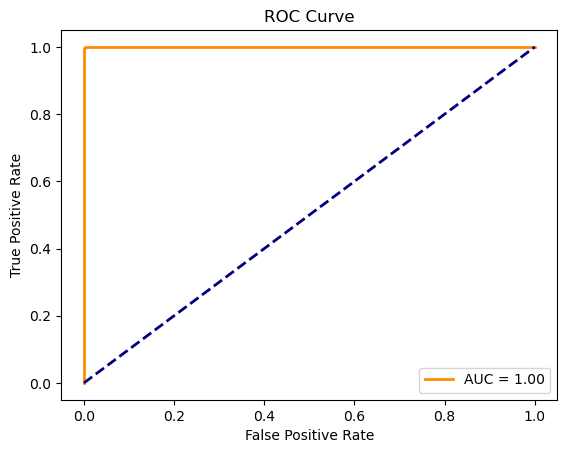
\includegraphics[width=0.5\linewidth]{./figures/ROC.png}
	\caption{Courbe ROC}
	\label{fig:ROC}
\end{figure}

Dans cette partie, nous avons construit un réseau neuronal convolutif performant capable de classer efficacement nos données par rapport à l’existence ou pas d’une transition de phase. L’architecture du modèle choisie permet d’extraire les caractéristiques complexes de nos données et l’entraînement a été optimisée pour cette tâche de classification binaire. Les métriques de notre modèle tel que la précision, la sensibilité, la matrice de confusion et la courbe ROC montrent la robustesse de notre modèle. Nous avons alors créé un modèle à la fois précis et efficace, qui démontre une performance exceptionnelle dans le classement des matrices du modèle Ising.

\addcontentsline{toc}{section}{Conclusion}
\section*{Conclusion}

\end{document}